\chapter{Preparation}
\label{ch.preparation}

\section{Calculate the depth resolution of the OCT-system performing the folloing steps}

\subsection{Calculate the central wavenumber $k_0$ and the broadness of the spectral envelope function $\Delta k$}

\begin{equation}
k_0=\frac{2\pi}{\lambda_0} \rightarrow \frac{\Delta k}{\Delta\lambda}=-\frac{2\pi}{\lambda_0^2} 
\label{eq:delta_k_herleitung}
\end{equation}

\begin{equation}
\|\Delta k\|=\frac{2\pi}{\lambda_0^2}\Delta\lambda
\label{eq:delta_k}
\end{equation}

With $\Delta\lambda = 130$~nm and $\lambda_0=1310~$nm equation \ref{eq:delta_k} becomes
\begin{equation}
k_0=\frac{2\pi}{1310~\mathrm{nm}}=4.80~\mathrm{\upmu m}^{-1}
\label{eq:k_0_wert}
\end{equation}
and
\begin{equation}
\|\Delta k\| = \frac{2\pi}{1310 ^2~\mathrm{nm}^2}\cdot130~\mathrm{nm}=0,48~\mathrm{\upmu m}^{-1}
\label{eq:delta_k_wert}
\end{equation}

\subsection{Calculate $\mathcal{F}\{S(k)\}=\breve{S}(z)$with respect to $P$}
The spectral power envelope $S(k)$ is a rectalngle of height $P$.
\begin{equation}
S(k)=P\cdot r_{\Delta k}(k-k_0)
\label{eq:S_k}
\end{equation}
with the rectangular function 

\begin{equation}
r_{\Delta k}(k-k_0)=\begin{cases}
1,&\mathrm{for}~|k-k_0|\leq\frac{\Delta k}{2} \\
0,&\mathrm{for}~|k-k_0|>\frac{\Delta k}{2} 
\end{cases}
\label{eq:rect}
\end{equation}

% A fourier transformation of $S(k)$ leads to $\breve{S}(z)$:
% \begin{equation}
% S(k)=P\cdot r_{\Delta k}(k-k_0)\qquad\laplace\qquad \mathrm{e}^{-jzk_0}\cdot P\Delta k\mathrm{sinc}(z\frac{\Delta k}{2})=\breve{S}(z)
% \label{eq:Transformation}
% \end{equation}
% with sinc$(x)=\frac{\mathrm{sin}(x)}{x}$
% 
% 
% \comwo{Nochmal ohne Korrespondenz, sondern selbst gerechnet:... �berleg dir ob was davon und wenn ja welches richtig ist}

% A Fourier transformation of $S(k)$ leads to $\breve{S}(z)$. To performe the Fourier transformation the function $Y(k)$ is introduced.
% \begin{equation}
% S(k)=P\cdot r_{\Delta k}(k-k_0)=Y(k-k_0)
% \label{eq:hilfsunktion}
% \end{equation} 
% 
% 
\begin{equation}
S(k)=Y(k-k_0)\qquad \laplace \qquad \breve{Y}(z)\cdot\mathrm{e}^{-jzk_0}=\breve{S}(z)
\label{eq:verschiebung}
\end{equation}

\begin{equation}
Y(k)=P\cdot r_{\Delta k}(k)
\label{eq:Y_k}
\end{equation}

To transform $Y(k)$ from the momentum space into the position-space the following integral needs to be solved:

\begin{equation} 
\begin{split} 
\breve{Y}(z)=\frac{1}{\sqrt{2\pi}}\int^{\infty}_{-\infty}P\cdot r_{\Delta k}(k)\mathrm{e}^{jkz}\mathrm{d}k \\
=			\frac{1}{\sqrt{2\pi}}\int^{\frac{\Delta k}{2}}_{-\frac{\Delta k}{2}}P\cdot \mathrm{e}^{jkz}\mathrm{d}k\\
=			\frac{P}{\sqrt{2\pi}}\left[\frac{\mathrm{e}^{jkz}}{jz}\right]^{\frac{\Delta k}{2}}_{-\frac{\Delta k}{2}}\\
=		\frac{P}{\sqrt{2\pi}}\left(\frac{\mathrm{e}^{j\Delta kz}}{jz}-\frac{\mathrm{e}^{-j\Delta kz}}{jz}\right)\\
=		\frac{P}{\sqrt{2\pi}}\cdot\frac{2\mathrm{sin}(\frac{\Delta k}{2}z)}{z}\\
=		\frac{P}{\sqrt{2\pi}}\Delta k \cdot\mathrm{sinc}(\frac{\Delta k}{2}z)
\end{split}
\end{equation}

with sinc$(x)=\frac{\mathrm{sin}(x)}{x}$

With equation \eqref{eq:verschiebung} this leads to

\begin{equation}
\breve{S}(z) = \frac{P}{\sqrt{2\pi}}\Delta k \cdot\mathrm{sinc}(\frac{\Delta k}{2}z)\cdot\mathrm{e}^{-jzk_0}
\label{eq:S_ortsraum}
\end{equation}

\subsection{What is the FWHM of $\breve{S}(z)$?}

To determine the Full Width Half Maximum (FWHM) of $\breve{S}(z)$ the Taylor series of sinc($x$) is used.

\begin{equation}
\begin{split}
\mathrm{sinc}(x)=\frac{\mathrm{sin}(x)}{x}=\sum^{\infty}_{n=0}{(-1)^n}{\frac{x^{2n}}{(2n+1)!}}\\
\approx 1-\frac{x^2}{3!}+\frac{x^4}{5!}.
\end{split}
\end{equation}
For the half width at half maximum $\breve{S}(z) = 0.5\cdot\breve{S}(0)$ must be solved.

The first positive zero of $1-\frac{x^2}{3!}+\frac{x^4}{5!}=0.5$ is 1.9. 
With $x=\frac{\Delta k}{2}z$ the result of the half width at half maximum is $8~\upmu$m. The FWHM is then $\delta l = 2\cdot 8~\upmu$m = 16~$\upmu$m. Figure \ref{fig:fwhm} shows the main peak of $\breve{S}(z)$ and the and the FWHM.

%The determination of the FWHM of $\breve{S}(z)$ was done graphical. Figure \ref{fig:fwhm} shows the main peak of $\breve{S}(z)$. The measured FWHM is $\sim$16~$\upmu$m. 
\begin{figure}[h]%
\centering
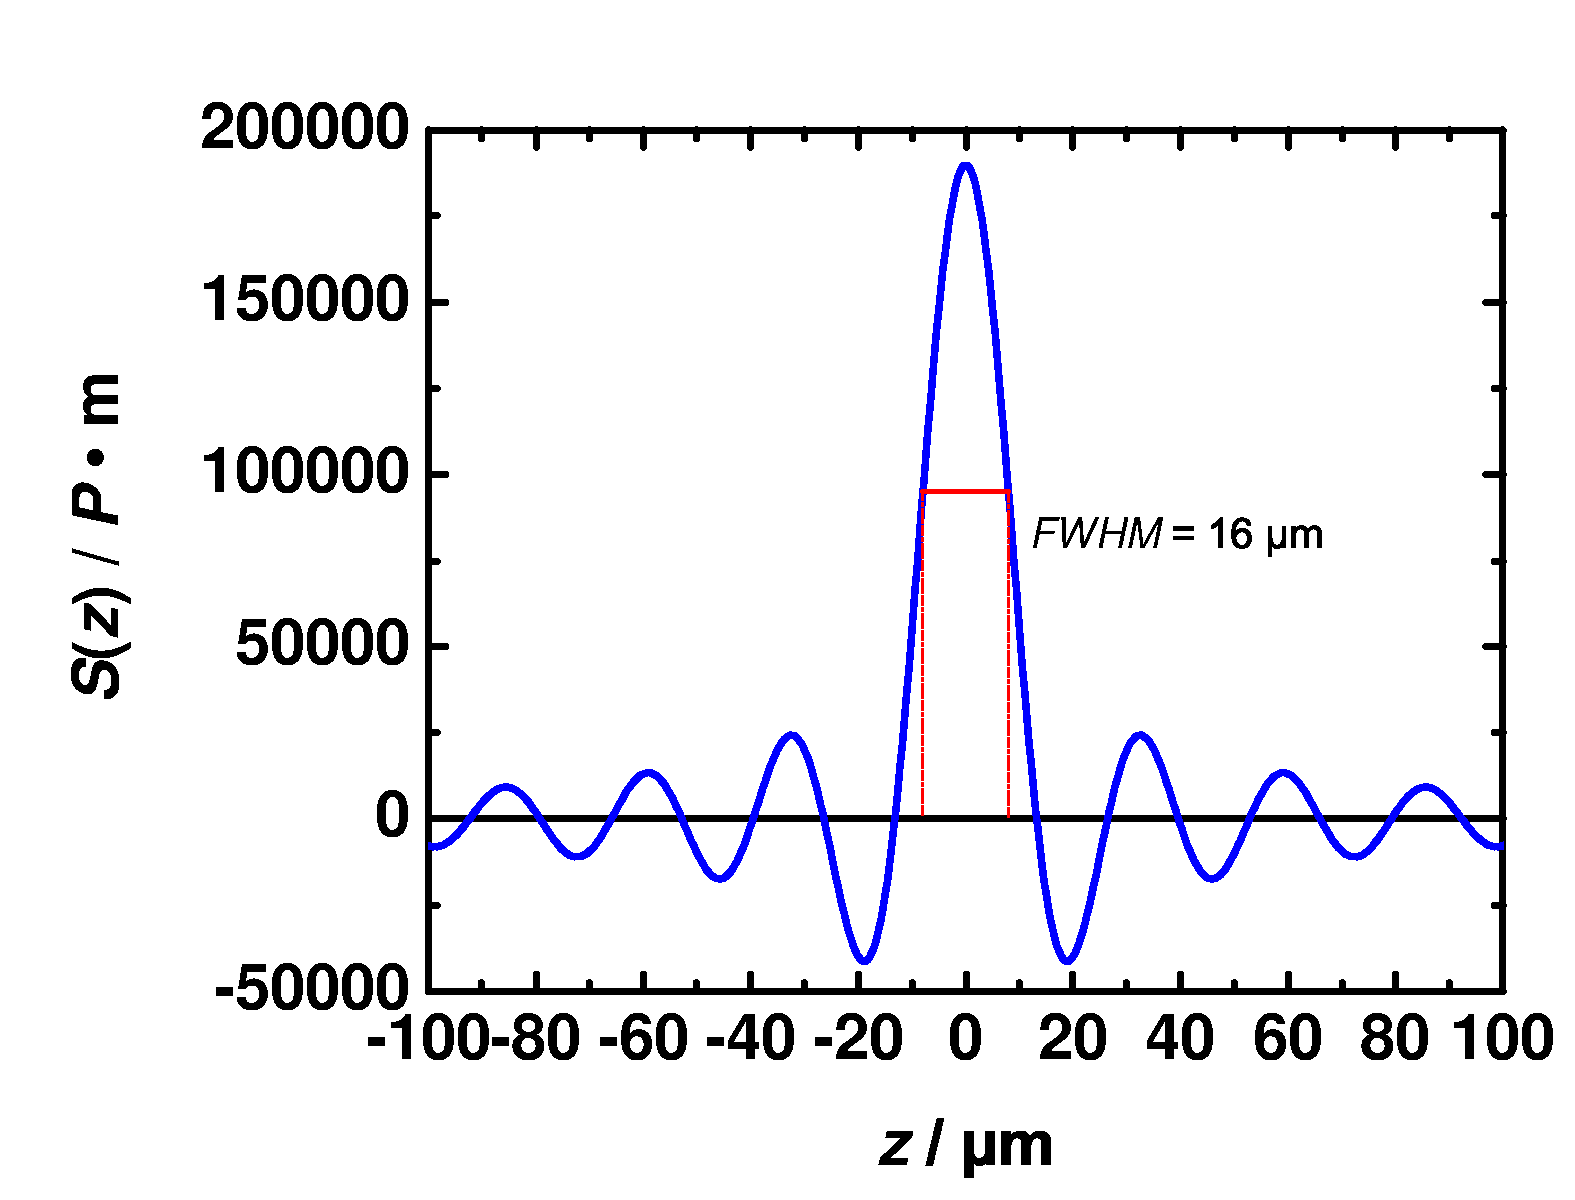
\includegraphics[width=.8\columnwidth]{Grafiken/FWHM_gros.pdf}
\caption{}%
\label{fig:fwhm}%

\end{figure}


\subsection{To which spatial resolution in $\upmu$m in z-coordinates does this correspond?}
Te resolve two points the peaks in the signal must be at least $\delta l$ apart. Because the light in the specimen travels the way to the reflecting plane and back in the medium with the refractive index $n$ the distance the light travels is $l=2\cdot nz$. From this follows that $\delta l = 2\cdot n\delta z$ and
\begin{equation}
\delta z = \frac{\delta l}{2n}=\frac{16~\upmu\mathrm{m}}{3} = 5.33~\upmu\mathrm{m}.
\label{eq:}
\end{equation}



\section{Calculate the depth profile of a spool of adhesive tape}

In a .mat file the measurement of the interface term of a spool of adhesive tape $\breve{u}(k_m)$ is given. The Values have been sampled with the interval $\delta k$ and are lineary spaced. To calculate the term in the spacial domain $\breve{u}(z)_{sr}$ the Matlab function \verb|fft()| is used. Now the spacing of the values in z space has to be calculated. This is done by
\begin{equation}
  \delta z = \frac{2\pi}{M\cdot \delta k}
\end{equation}
where $M$ is the total number of values given in the file. Like in \ref{sec:resolution} it has to be taken into account, that the light measured at the detector travels back and forth through the sample. Also the refractive index of the sample can not be neglegted. With \eqref{eq:resolution} follows
\begin{equation}
  \delta z = \frac{2\pi}{2n\cdot M\cdot \delta k}.
\end{equation}
This calculation is also done with Matlab. The absolute of $\breve{u}(z)_{sr}$ is shown in fig. \ref{fig:profile}. Since $\breve{u}(z)_{sr}$ is symmetric around $z=4$~mm only the range 4~mm$~\leq z\leq~$8~mm is plotted.

Most noticable in figure \ref{fig:profile} is a large peak around $z=1.6$~mm and the increasing of $I$ for $z \rightarrow 0$~mm. This increasing of $I$ towards 0~mm are DC parts caused by non-interfering components. 
At $z\approx1.6$~mm the signal shows a good reflecting plane. Figure \ref{fig:profile_zoom} shows the range from 1.4 to 2.5~mm. Here the layer thickness of the tape can be approximated. 


\begin{figure}[ht]
  \centering
  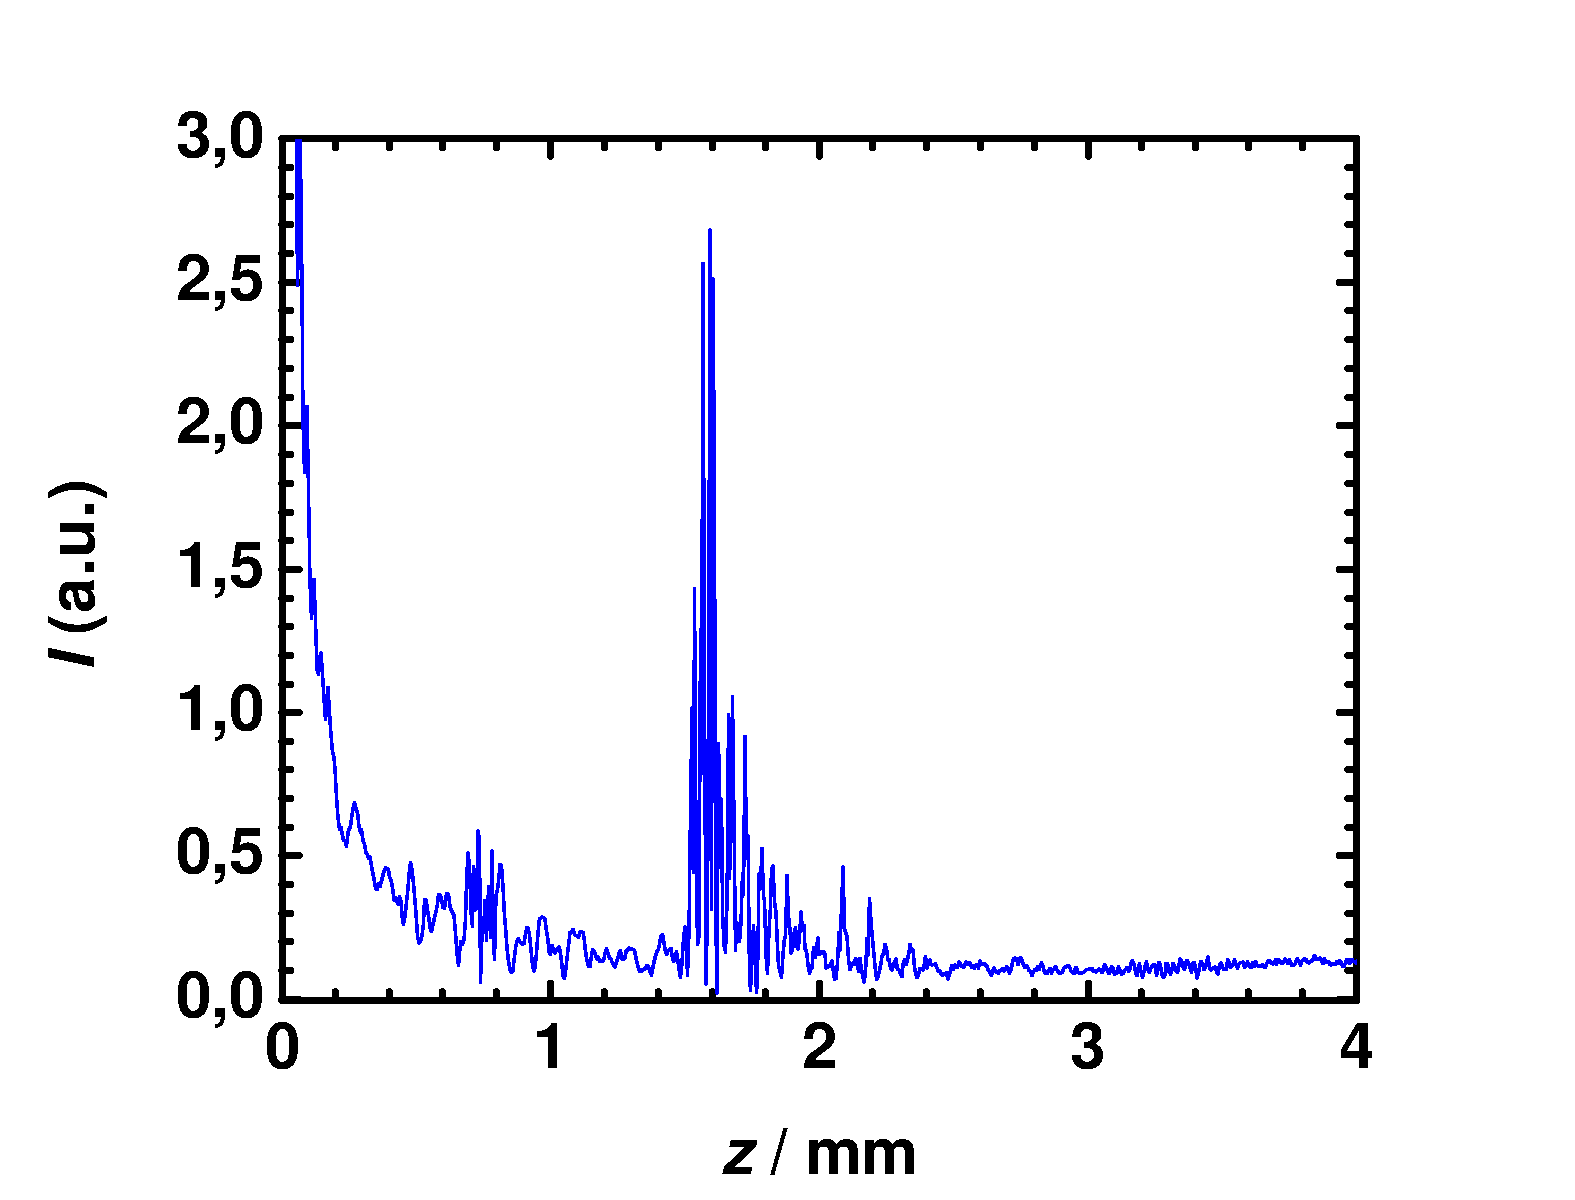
\includegraphics[width=.6\columnwidth]{Grafiken/profile_mm_2.pdf}

\caption{ }
\label{fig:profile}
\end{figure}


\begin{figure}[ht]
  \centering
  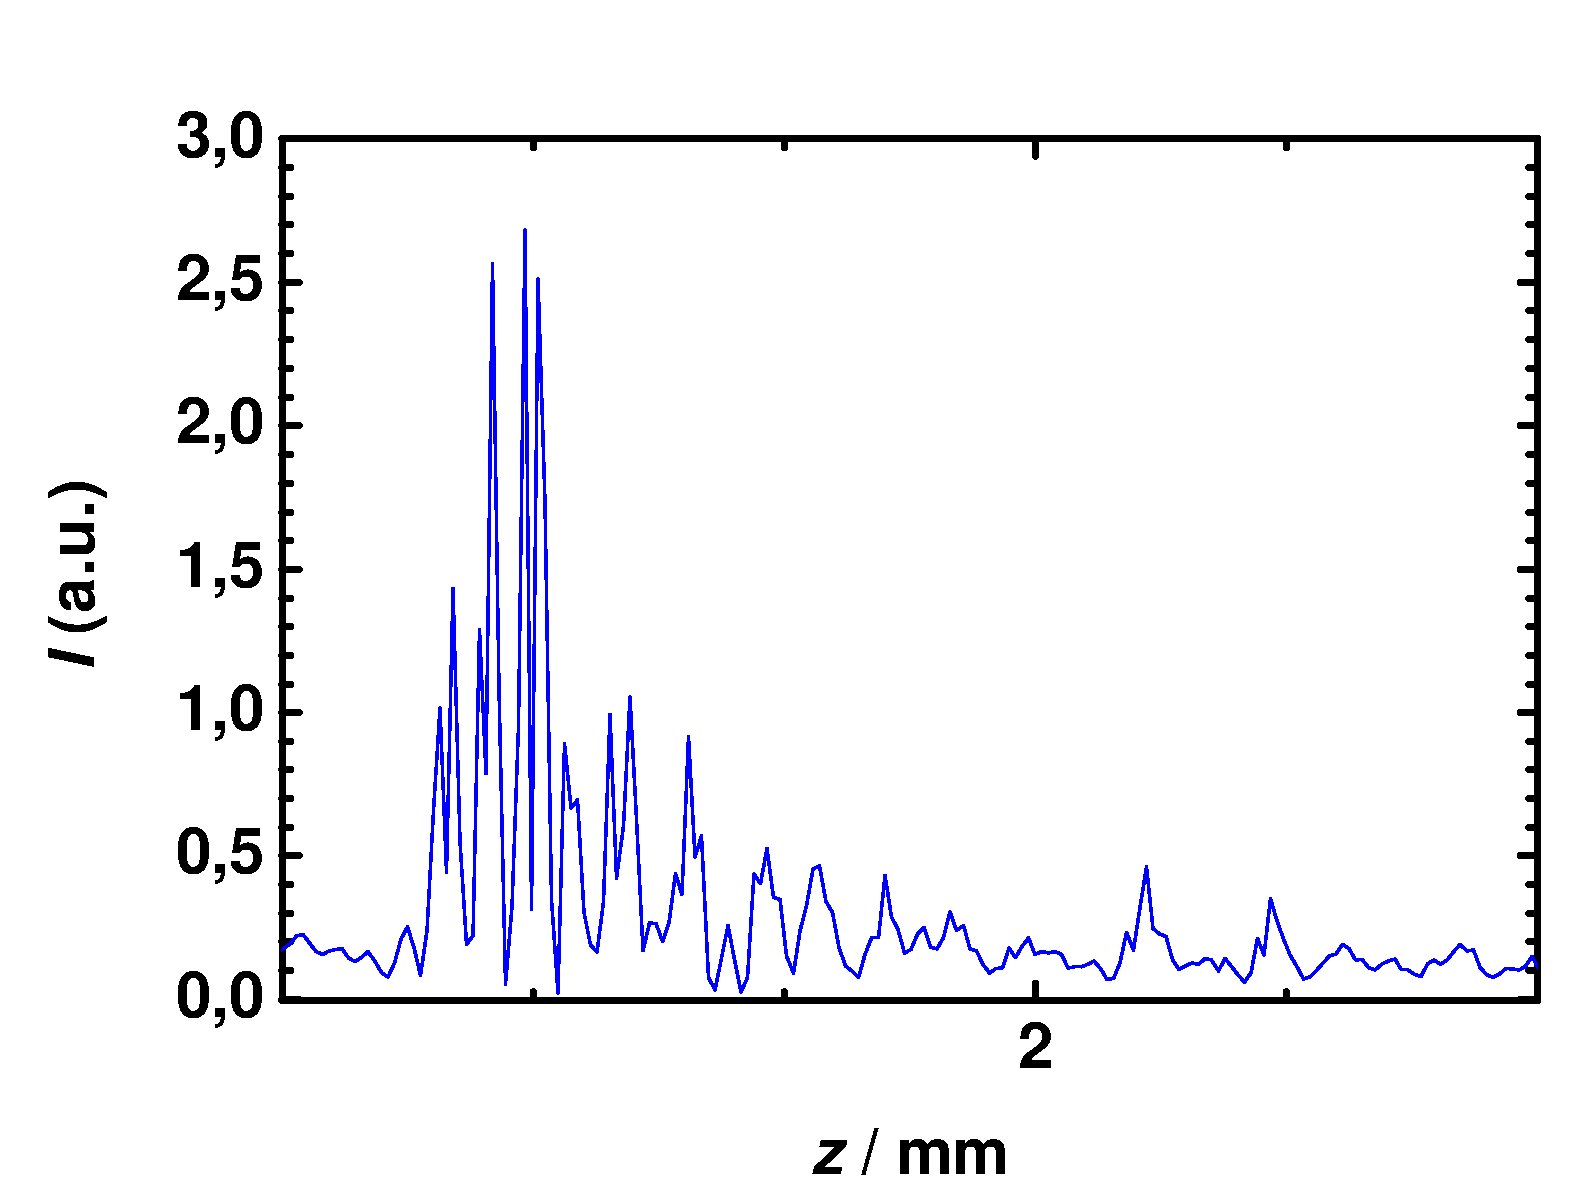
\includegraphics[width=.6\columnwidth]{Grafiken/profile_14-24.pdf}

\caption{ }
\label{fig:profile_zoom}
\end{figure}
